% =====================================================================
% Notas de presentación · GA-TL-01 · Grupo CMSZ
% Cooperativa Ahorro Futuro · Escenario 4
% Responsable del documento: S (Sánchez Vera Darwin Joel)
%
% Fuentes de cada sección (si el dueño cambia su ficha, se actualiza aquí):
%   Matriz de interacciones ...... docs/matriz-interacciones.md (C)
%   Flujos 1 y 2 ................. docs/flujos/flujo-1.md, flujo-2.md (C)
%   Flujos 4 y 5 ................. docs/flujos/flujo-4.md, flujo-5.md (M)
%   Flujos 3 y 6 ................. docs/flujos/flujo-3.md, flujo-6.md (S)
%   Flujos 7 y 8 ................. sección LaTeX entregada por Z (pegada sin cambios)
%   Diagrama ..................... ../diagrama/sistema-bancario.png (M)
%
% Compilar desde la carpeta notas/:
%   pdflatex notas-presentacion.tex   (dos veces)
%   o bien: latexmk -pdf notas-presentacion.tex
% =====================================================================
\documentclass[11pt,a4paper]{article}
\usepackage[T1]{fontenc}
\usepackage[utf8]{inputenc}
\usepackage[spanish,es-tabla,es-noshorthands]{babel}
\usepackage{lmodern}
\usepackage[a4paper,margin=2cm]{geometry}
\usepackage{graphicx}
\usepackage{array}
\usepackage{longtable}
\usepackage{pdflscape}
\usepackage[hidelinks]{hyperref}

\graphicspath{{../diagrama/}}
\setlength{\parindent}{0pt}
\setlength{\parskip}{4pt}
\newcolumntype{P}[1]{>{\raggedright\arraybackslash}p{#1}}

\title{\textbf{Notas de presentación}\\[4pt]
\large GA-TL-01 · Taller de modelado de comunicación entre procesos distribuidos\\
Escenario 4: Cooperativa Ahorro Futuro · Grupo CMSZ}
\author{C: Cedeño Intriago Jilmar Jesús \and M: Mendoza Bermello Angello Agustín \\
        S: Sánchez Vera Darwin Joel \and Z: Zambrano Triviño Leonel Leonidas}
\date{Aplicaciones Distribuidas (ISR-701) · Entrega: miércoles 11/11/2026}

\begin{document}
\maketitle

% =====================================================================
\section{Escenario y requisitos}
% =====================================================================
Cooperativa Ahorro Futuro es una cooperativa de ahorro y crédito con agencias en Los Ríos y
Guayas. Sus socios usan banca web, cajeros automáticos propios y ventanillas. Los saldos viven en
un core bancario heredado que no se puede reemplazar a corto plazo. En los días de pago las
transferencias se demoran, hay débitos duplicados cuando el socio pulsa dos veces «enviar» y
algunos cajeros entregan dinero sin que el débito quede registrado.

\textbf{Actores:} socio, cajero de ventanilla, cajero automático, analista de fraude y red
interbancaria.

\textbf{Operaciones modeladas:} (a) notificar el movimiento al socio y registrarlo en auditoría;
(b) transferir entre cuentas de la cooperativa; (c) transferir a otro banco por la red
interbancaria; (d) retirar efectivo en un cajero automático; (e) consultar el saldo.

\subsection*{Requisitos R1--R6 y cómo los cumple el diseño}

\begin{center}
\small
\begin{tabular}{|l|P{4.6cm}|P{7.2cm}|P{1.6cm}|}
\hline
\textbf{Req.} & \textbf{Qué exige} & \textbf{Cómo se cumple} & \textbf{Flujos} \\ \hline
R1 & 300 transacciones por segundo en días de pago; el 95\,\% en menos de 2 s &
     gRPC/HTTP2, pooling, cola RabbitMQ que absorbe picos y prueba de carga & 1, 7 \\ \hline
R2 & El saldo se confirma en el core; nunca se debita dos veces la misma operación &
     Idempotency key + restricción única + estado de operación & 3, 5 \\ \hline
R3 & Antifraude responde en menos de 200 ms; el equipo define qué hacer si no responde &
     Deadline de 200 ms + circuit breaker + política de contingencia & 2 \\ \hline
R4 & Cajeros con mensajes de formato fijo y timeout máximo de 15 s; sin respuesta no entregan dinero &
     Sockets TCP, framing, formato fijo y timeout de 15 s & 4 \\ \hline
R5 & Toda operación queda en auditoría, aunque el servicio de auditoría esté caído &
     Outbox transaccional + Kafka durable + reintentos & 8 \\ \hline
R6 & Disponibilidad del 99,95\,\% para transferencias y retiros &
     Réplicas, health checks, reintentos con backoff y degradación graceful & 2, 6, 7, 8 \\ \hline
\end{tabular}
\end{center}

% =====================================================================
\begin{landscape}
\section{Diagrama de comunicación}
\IfFileExists{../diagrama/sistema-bancario.png}{%
\begin{center}
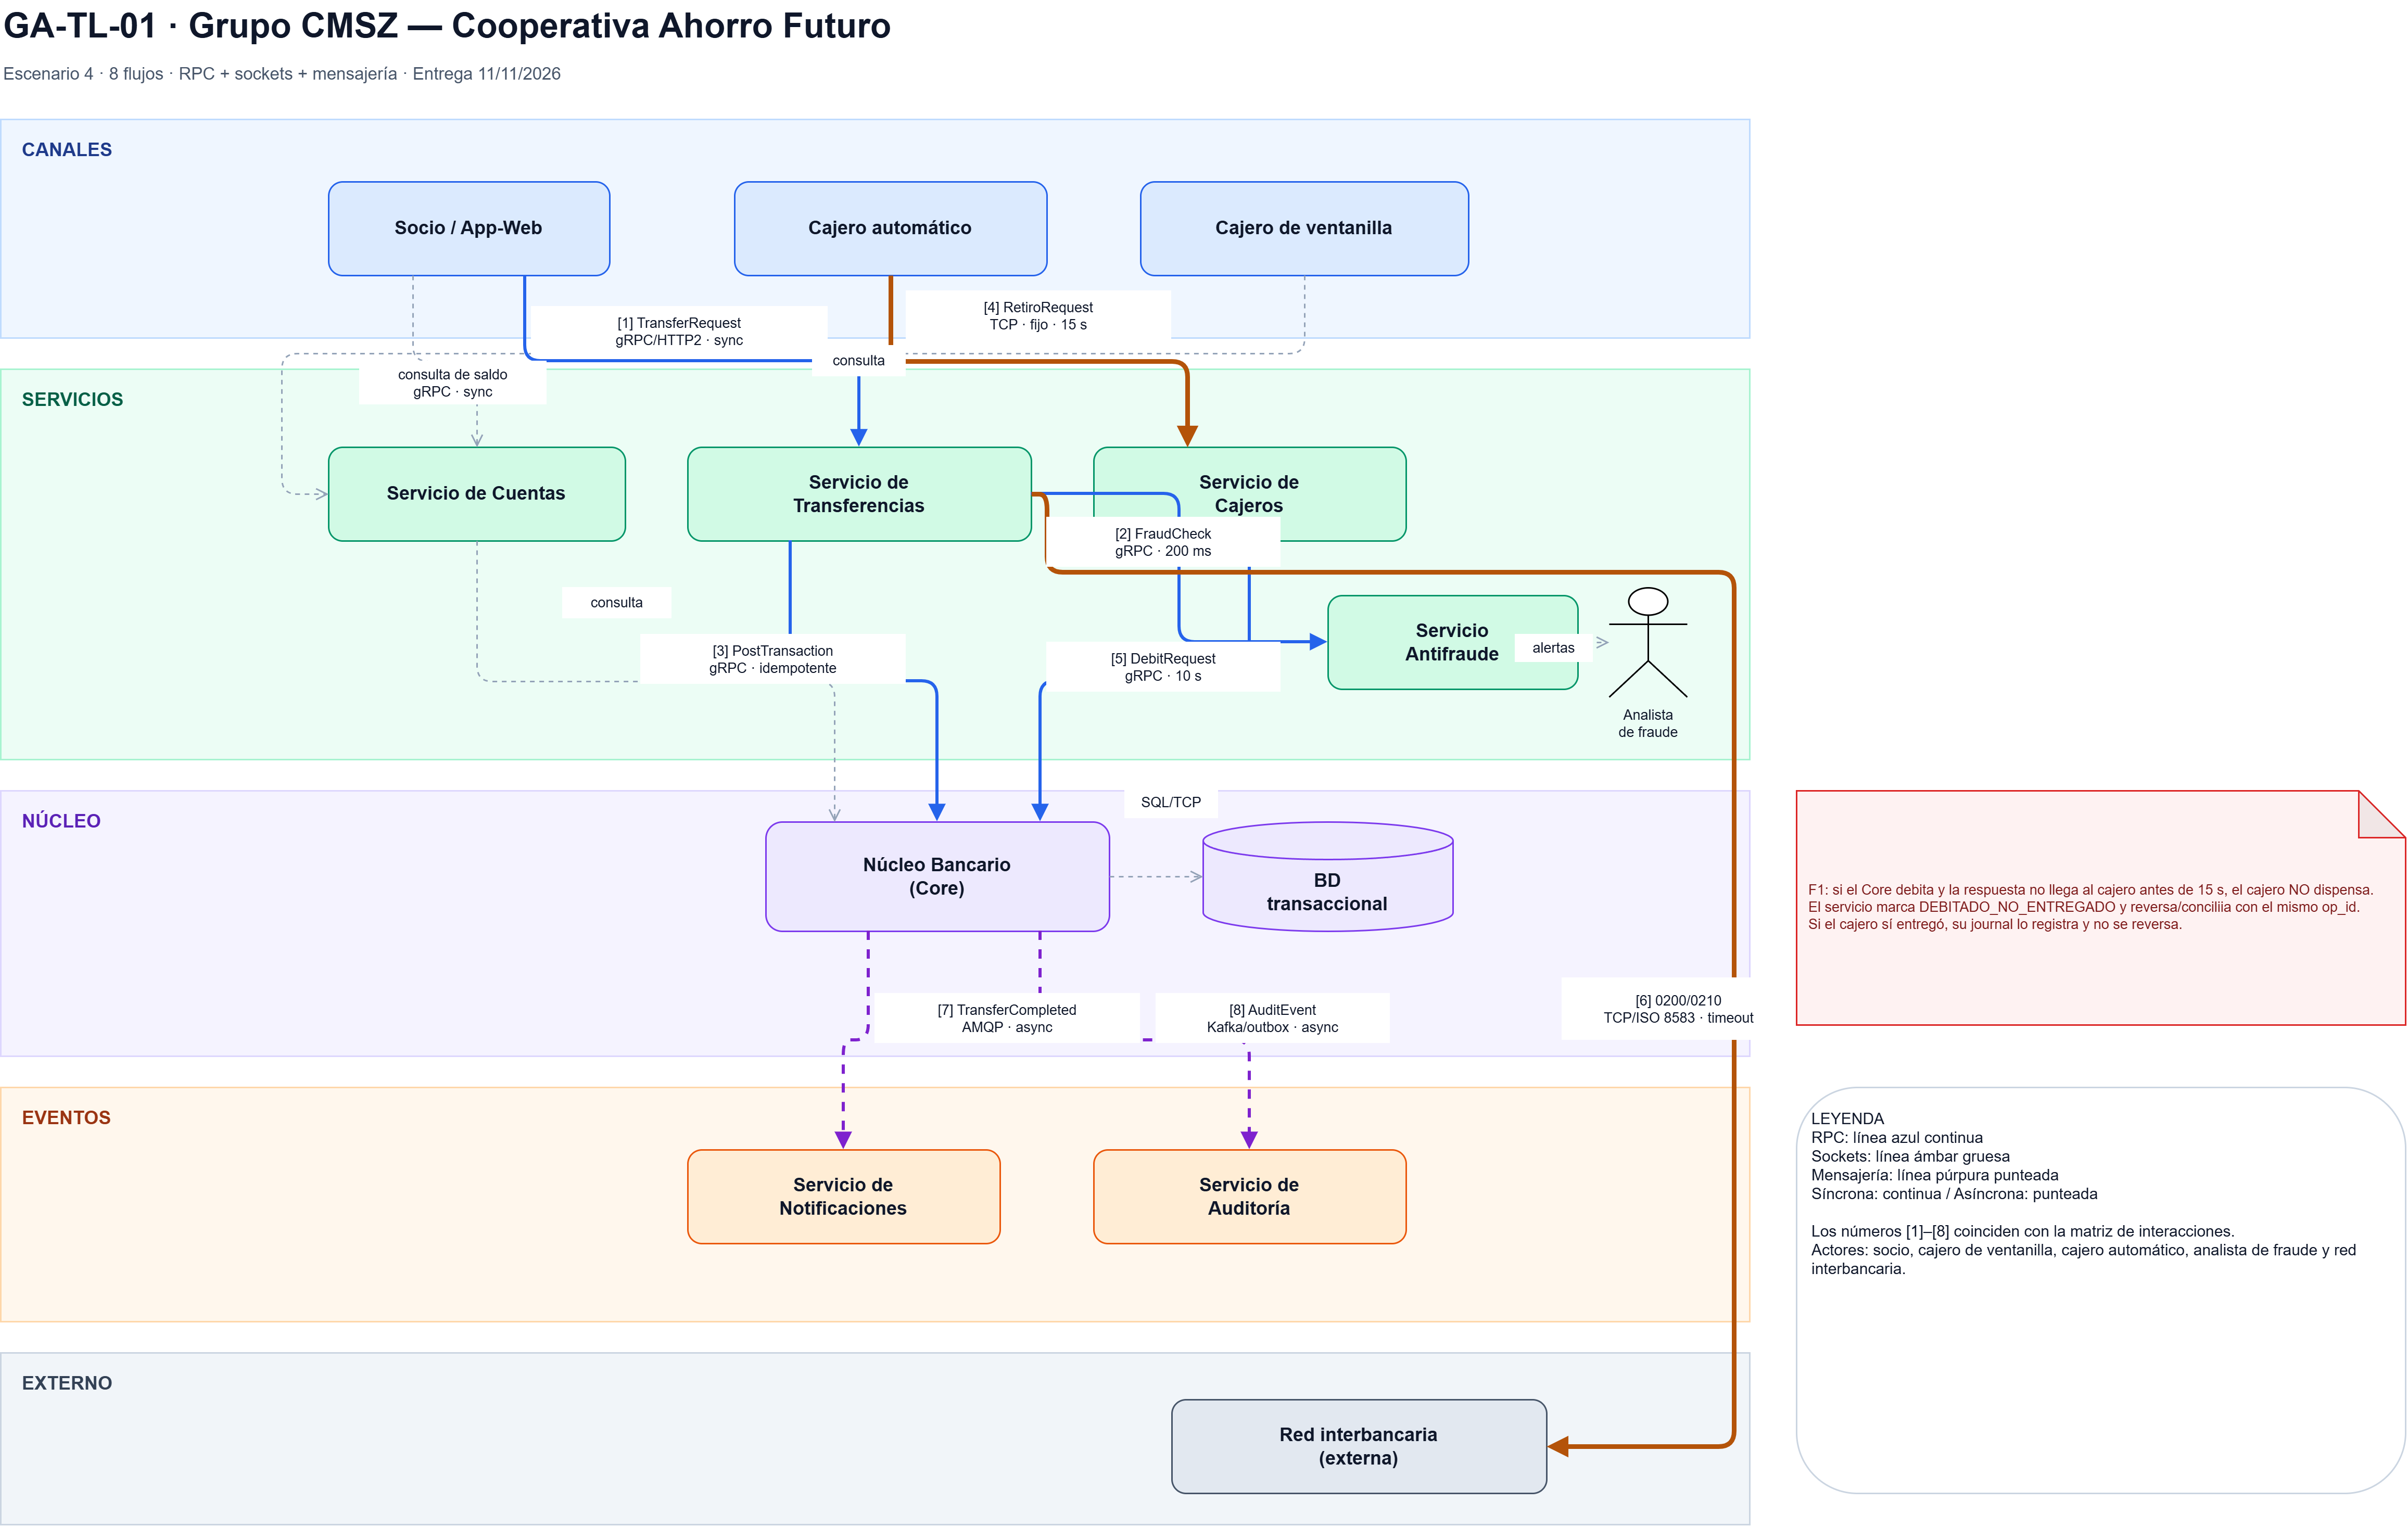
\includegraphics[width=\linewidth,height=0.78\textheight,keepaspectratio]{sistema-bancario.png}
\end{center}}{\textit{(Falta la exportación del diagrama: diagrama/sistema-bancario.png.)}}

Archivo editable: \texttt{diagrama/sistema-bancario.drawio}. Los números [1]--[8] de las
flechas coinciden con la matriz de interacciones de la sección~\ref{sec:matriz}.
\end{landscape}

% =====================================================================
\begin{landscape}
\section{Matriz de interacciones}\label{sec:matriz}
{\small
\setlength{\tabcolsep}{4pt}
\begin{longtable}{|c|P{2.7cm}|P{2.6cm}|P{1.7cm}|P{2.3cm}|P{4.4cm}|P{7.0cm}|c|}
\hline
\textbf{\#} & \textbf{Origen} & \textbf{Destino} & \textbf{Tipo} & \textbf{Sync/Async} &
\textbf{Protocolo / middleware} & \textbf{Justificación y requisito} & \textbf{Dueño} \\ \hline
\endhead
1 & App/Web & Servicio de Transferencias & RPC & Síncrona & gRPC-Web sobre HTTP/2 &
  El socio requiere respuesta inmediata; contrato tipado y multiplexación para 300 TPS y p95
  menor de 2 s (R1). La solicitud conserva una clave de idempotencia (R2). & C \\ \hline
2 & Servicio de Transferencias & Servicio Antifraude & RPC & Síncrona; deadline de 200 ms &
  gRPC sobre HTTP/2, deadline y circuit breaker &
  El análisis debe anteceder al débito (R3). Ante una caída se aplica contingencia diferenciada,
  sin detener todas las operaciones (R6). & C \\ \hline
3 & Servicio de Transferencias & Core bancario & RPC & Síncrona &
  gRPC sobre HTTP/2, adaptador del core, idempotency key y pool de conexiones &
  Solo el core confirma saldos oficiales; la misma operación no genera doble débito (R2). & S \\ \hline
4 & Cajero automático & Servicio de Cajeros & Sockets & Síncrona; timeout máximo de 15 s &
  TCP, mensajes de formato fijo, framing length-prefix; mTLS opcional &
  El dispositivo heredado usa formato fijo y no entrega efectivo sin confirmación (R4). & M \\ \hline
5 & Servicio de Cajeros & Core bancario & RPC & Síncrona; deadline de 10 s &
  gRPC sobre HTTP/2 con idempotencia &
  El adaptador consulta al sistema de registro y confirma el débito antes de autorizar la
  entrega de efectivo (R2, R4). & M \\ \hline
6 & Servicio de Transferencias & Red interbancaria & Sockets & Síncrona; timeout controlado &
  TCP y mensajes de formato fijo (supuesto: ISO 8583) &
  Se integra una red externa heredada, con estados de proceso, conciliación y compensación ante
  incertidumbre (R6). & S \\ \hline
7 & Transferencias / Core (publica el relay del outbox) & Servicio de Notificaciones & Mensajería &
  Asíncrona & AMQP 0-9-1 con RabbitMQ; reintentos y DLQ &
  El socio no espera el envío de SMS o correo; la cola absorbe picos y permite reintentos
  (R1, R6). & Z \\ \hline
8 & Core / Transferencias & Servicio de Auditoría & Mensajería & Asíncrona &
  Kafka y outbox transaccional; clave de partición \texttt{cuenta} &
  El evento persiste aunque auditoría no esté disponible y se entrega después (R5). & Z \\ \hline
\end{longtable}
}
\end{landscape}

% =====================================================================
\section{Flujos por responsable}
% =====================================================================
Cada integrante modeló y justificó dos flujos. En cada ficha se indica el tipo de comunicación,
si es síncrona o asíncrona, el protocolo o middleware, el mensaje y los requisitos que atiende.

% ---------------------------------------------------------------------
\subsection{Canal del socio y antifraude (Flujos 1 y 2)}
% Fuente: docs/flujos/flujo-1.md y flujo-2.md (C)

\subsubsection*{Flujo 1 --- App/Web $\rightarrow$ Servicio de Transferencias}

\begin{tabular}{|l|p{9.5cm}|}
\hline
\textbf{Tipo} & RPC \\ \hline
\textbf{Sync/Async} & Síncrona \\ \hline
\textbf{Protocolo} & gRPC-Web sobre HTTP/2 \\ \hline
\textbf{Mensaje} & \texttt{TransferRequest\{idempotency\_key, cuenta\_origen, cuenta\_destino, monto, moneda\}} \\ \hline
\textbf{Requisitos} & R1, R2 \\ \hline
\textbf{Dueño} & C \\ \hline
\end{tabular}

\medskip
\textbf{Por qué.} El socio necesita conocer el resultado al confirmar la transferencia. El
contrato tipado de gRPC define el mensaje y su respuesta, y HTTP/2 permite multiplexar
solicitudes para la meta de 300 TPS con p95 menor de 2 s (R1). La misma
\texttt{idempotency\_key} se conserva en los reintentos (R2). Para un navegador, gRPC-Web puede
requerir un proxy compatible; es un supuesto de despliegue, no una interacción nueva.

\textbf{Si falla.} Si se interrumpe la comunicación o vence el tiempo de espera, la interfaz no
asume éxito ni fracaso: muestra \texttt{PENDIENTE} y cualquier consulta o reintento usa la misma
\texttt{idempotency\_key}; nunca se generan dos débitos.

\subsubsection*{Flujo 2 --- Servicio de Transferencias $\rightarrow$ Servicio Antifraude}

\begin{tabular}{|l|p{9.5cm}|}
\hline
\textbf{Tipo} & RPC \\ \hline
\textbf{Sync/Async} & Síncrona; deadline de 200 ms \\ \hline
\textbf{Protocolo} & gRPC sobre HTTP/2, deadline de 200 ms y circuit breaker \\ \hline
\textbf{Mensaje} & \texttt{FraudCheckRequest\{op\_id, cuenta, monto, beneficiario, canal\}}
                   $\rightarrow$ \texttt{APROBAR | RECHAZAR | REVISAR} \\ \hline
\textbf{Requisitos} & R3, R6 \\ \hline
\textbf{Dueño} & C \\ \hline
\end{tabular}

\medskip
\textbf{Por qué.} La revisión de riesgo debe ocurrir antes del débito en el core. R3 exige
respuesta en menos de 200 ms, y una llamada gRPC síncrona permite fijar ese deadline. Como la
dependencia síncrona puede afectar la disponibilidad, un circuit breaker limita las llamadas a un
servicio inestable y activa la contingencia (R6).

\textbf{Si falla (F2).} Ni se detienen todas las transferencias ni se aprueban sin revisión: las
de monto bajo sin alertas continúan marcadas para revisión posterior; las de monto alto o riesgo
elevado quedan en \texttt{PENDIENTE\_REVISION}. Toda decisión de contingencia queda registrada
para auditoría. El umbral entre monto bajo y alto no está definido en la actividad y corresponde
a una política institucional.

% ---------------------------------------------------------------------
\subsection{Cajero automático y sockets (Flujos 4 y 5)}
% Fuente: docs/flujos/flujo-4.md y flujo-5.md (M)

\subsubsection*{Flujo 4 --- Cajero automático $\rightarrow$ Servicio de Cajeros}

\begin{tabular}{|l|p{9.5cm}|}
\hline
\textbf{Tipo} & Sockets TCP \\ \hline
\textbf{Sync/Async} & Síncrona; timeout de 15 s \\ \hline
\textbf{Protocolo} & TCP con framing length-prefix, formato fijo y mTLS opcional \\ \hline
\textbf{Mensaje} & \texttt{RetiroRequest}, formato fijo:\newline \texttt{[len][ver][tipo][tarjeta][monto]}\newline \texttt{[cajero\_id][op\_id][crc]} \\ \hline
\textbf{Requisitos} & R4, R6 \\ \hline
\textbf{Dueño} & M \\ \hline
\end{tabular}

\medskip
\textbf{Por qué.} R4 exige formato fijo y timeout de 15 s. El cajero es legacy; los sockets TCP
permiten controlar el framing, la conexión persistente y el timeout. No se dispensa sin
respuesta.

\textbf{Si falla.} Sin respuesta en 15 s el cajero no dispensa; la operación queda
\texttt{EN\_PROCESO} y se consulta o revierte con el \texttt{op\_id}; luego se concilia. Estados
de la operación: \texttt{INICIADA}, \texttt{DEBITADA}, \texttt{ENTREGADA},
\texttt{DEBITADO\_NO\_ENTREGADO}, \texttt{REVERSADA} y \texttt{EN\_PROCESO}.

\subsubsection*{Flujo 5 --- Servicio de Cajeros $\rightarrow$ Core}

\begin{tabular}{|l|p{9.5cm}|}
\hline
\textbf{Tipo} & RPC (gRPC) \\ \hline
\textbf{Sync/Async} & Síncrona; deadline de 10 s \\ \hline
\textbf{Protocolo} & gRPC/HTTP2 con idempotencia y deadline de 10 s \\ \hline
\textbf{Mensaje} & \texttt{DebitRequest\{op\_id, tarjeta, monto, cajero\_id\}} \\ \hline
\textbf{Requisitos} & R2, R4 \\ \hline
\textbf{Dueño} & M \\ \hline
\end{tabular}

\medskip
\textbf{Por qué.} El servicio de cajeros actúa como adaptador: recibe el formato fijo por socket
y llama al core por gRPC. El débito se confirma antes de que el cajero entregue dinero, y la
idempotencia protege los reintentos. El deadline de 10 s deja margen dentro de los 15 s del
cajero.

\textbf{Si falla.} Si el core no responde en 10 s, el servicio responde \texttt{NO\_DISPENSAR}:
el cajero no entrega dinero, la operación se marca \texttt{EN\_PROCESO} y se revierte o concilia.

% ---------------------------------------------------------------------
\subsection{Núcleo y red interbancaria (Flujos 3 y 6)}
% Fuente: docs/flujos/flujo-3.md y flujo-6.md (S)

El core es el sistema de registro: ninguna transferencia se da por hecha hasta que el core la
confirma, y la misma operación nunca se debita dos veces (R2). El \texttt{op\_id} identifica la
operación en todos los flujos que la tocan, incluidos los reintentos, la reversa y la
conciliación.

\subsubsection*{Flujo 3 --- Servicio de Transferencias $\rightarrow$ Core}

\begin{tabular}{|l|p{9.5cm}|}
\hline
\textbf{Tipo} & RPC \\ \hline
\textbf{Sync/Async} & Síncrona \\ \hline
\textbf{Protocolo} & gRPC/HTTP2 hacia el adaptador gRPC del core, con idempotency key y pool de conexiones \\ \hline
\textbf{Mensaje} & \texttt{PostTransaction\{op\_id, débito, crédito, monto\}} \\ \hline
\textbf{Requisitos} & R2, R1 \\ \hline
\textbf{Dueño} & S \\ \hline
\end{tabular}

\medskip
\textbf{Por qué.} El saldo oficial vive en el core. Transferencias necesita una confirmación
síncrona antes de responder al socio, y el débito y el crédito deben quedar en una sola
transacción: consistencia fuerte. gRPC/HTTP2 aporta contrato tipado y deadline; el pool de
conexiones reutiliza las conexiones con el adaptador para el pico de 300 TPS (R1). La restricción
única sobre \texttt{op\_id} evita el doble débito (R2).

\textbf{Secuencia.}
\begin{enumerate}
  \item Con la aprobación de antifraude (flujo 2), Transferencias envía \texttt{PostTransaction}
        con \texttt{op\_id}, las cuentas de débito y crédito y el monto.
  \item El core valida la restricción única de \texttt{op\_id}.
  \item Si el \texttt{op\_id} es nuevo, debita y acredita en una sola transacción; en esa misma
        transacción quedan en el outbox los eventos de la operación (flujos 7 y 8).
  \item Si el \texttt{op\_id} ya existe, devuelve el resultado original sin debitar otra vez.
  \item El core responde OK o error; Transferencias actualiza el estado y responde al canal.
\end{enumerate}

\textbf{Si falla.} Ante un timeout o una respuesta perdida, la operación queda
\texttt{PENDIENTE}: Transferencias consulta al core por \texttt{op\_id} y, si reintenta, lo hace
con el mismo \texttt{op\_id}, de modo que el core devuelve el resultado original. Si el estado
sigue incierto, la conciliación lo resuelve con el mismo identificador.

\textbf{Trade-off.} Ganamos consistencia fuerte y débito único. Pagamos que la transferencia
depende de que el core responda y que un timeout deja un estado incierto que obliga a consultar y
conciliar.

\subsubsection*{Flujo 6 --- Servicio de Transferencias $\rightarrow$ Red interbancaria}

\begin{tabular}{|l|p{9.5cm}|}
\hline
\textbf{Tipo} & Sockets \\ \hline
\textbf{Sync/Async} & Síncrona, con timeout \\ \hline
\textbf{Protocolo} & TCP con mensajes de formato fijo (supuesto: ISO 8583) \\ \hline
\textbf{Mensaje} & 0200/0210 · \texttt{op\_id}, monto, beneficiario, banco destino \\ \hline
\textbf{Requisitos} & R6, R2 \\ \hline
\textbf{Dueño} & S \\ \hline
\end{tabular}

\medskip
\textbf{Por qué.} La red interbancaria es externa y legacy: no se controla su latencia ni se
puede cambiar su protocolo, así que no se usa gRPC sino el formato fijo que la red expone
(supuesto: ISO 8583 sobre TCP; 0200 es la solicitud y 0210 la respuesta). Un timeout corto evita
que Transferencias quede bloqueado por una red lenta: la operación queda \texttt{EN\_PROCESO} y se
resuelve después (R6). Si la red rechaza, el débito se compensa (R2).

\textbf{Secuencia.}
\begin{enumerate}
  \item El débito de la cuenta del socio ya quedó registrado en el core por el flujo 3; por eso un
        rechazo se corrige con una reversa.
  \item Transferencias envía 0200 con \texttt{op\_id}, monto, beneficiario y banco destino.
  \item La red responde 0210 con aprobación o rechazo.
  \item Si aprueba, se confirma la operación y se notifica al socio.
  \item Si rechaza, se reversa el débito con el mismo \texttt{op\_id}.
  \item Si no responde dentro del timeout, queda \texttt{EN\_PROCESO}, se reintenta con el mismo
        \texttt{op\_id} y se concilia.
\end{enumerate}

\textbf{Trade-off.} Ganamos integración con un sistema que no controlamos sin bloquear el
servicio. Pagamos el manejo de framing y formato fijo, un estado intermedio visible para el
socio y un proceso de conciliación.

% ---------------------------------------------------------------------
% Sección de Z (Zambrano Triviño Leonel Leonidas), pegada sin cambios.
% ============================================================
% Sección de Z — Flujos 7 y 8 (eventos) — versión 2
% Para pegar en notas/notas-presentacion.tex
% Solo usa tabular y \textbf: no requiere paquetes extra.
% Cambios respecto a la ficha original:
%  - Flujo 7: mensaje MovimientoRegistrado, lo publica el relay del outbox.
%  - Flujo 8: outbox en la BD transaccional y en Transferencias;
%    dedup por (op_id, tipo); partición por cuenta; relay corregido.
% ============================================================

\subsection{Eventos: notificaciones y auditoría (Flujos 7 y 8)}

Notificaciones y auditoría son procesos de eventos: asíncronos, toleran
reintentos y no bloquean la operación principal. Ambos parten de una misma
fuente, la tabla \emph{outbox}, donde cada operación deja su evento dentro de
la misma transacción que la registra. Un relay lee el outbox y publica en dos
middleware distintos, porque resuelven problemas distintos: RabbitMQ como cola
de trabajo con reintentos y DLQ para avisar al socio, y Kafka como registro
durable y re-legible para la auditoría.

\subsubsection*{Flujo 7 --- Transferencias / Core $\rightarrow$ Notificaciones}

\begin{tabular}{|l|p{9.5cm}|}
\hline
\textbf{Tipo} & Mensajería \\ \hline
\textbf{Sync/Async} & Asíncrona \\ \hline
\textbf{Middleware} & AMQP 0-9-1 con RabbitMQ; reintentos y DLQ \\ \hline
\textbf{Publica} & Relay del outbox (carril Núcleo) \\ \hline
\textbf{Mensaje} & \texttt{MovimientoRegistrado\{op\_id, cuenta, monto, canal, tipo\}} \\ \hline
\textbf{Requisitos} & R1, R6 \\ \hline
\textbf{Dueño} & Z \\ \hline
\end{tabular}

\medskip
\textbf{Por qué.} El socio no necesita esperar a que se envíe el SMS, el
correo o la push. RabbitMQ desacopla el pico de 300 TPS de los días de pago
(R1), permite reintentos y envía a DLQ los mensajes que no se pueden entregar.
Publicar desde el outbox, y no desde Transferencias, evita perder avisos si un
proceso cae justo después de que el core confirma, y cubre todo movimiento que
pasa por el core: transferencias, retiros en cajero y reversas (operación a).

\textbf{Secuencia.}
\begin{enumerate}
  \item La operación y su evento quedan en el outbox, en la misma transacción.
  \item El relay publica \texttt{MovimientoRegistrado} en el exchange de RabbitMQ.
  \item RabbitMQ enruta el mensaje a la cola de notificaciones.
  \item El consumidor de notificaciones envía SMS, correo o push.
  \item Si el envío falla, se reintenta; agotados los reintentos, el mensaje
        pasa a la DLQ.
  \item La operación nunca espera la notificación.
\end{enumerate}

\textbf{Si falla.} Si notificaciones cae, el mensaje queda en la cola (durable,
con mensajes persistentes). Si RabbitMQ no está disponible, el evento espera en
el outbox y el relay reintenta. En ningún caso se detiene la operación (R6).

\textbf{Trade-off.} Ganamos desacoplamiento, absorción de picos y avisos que no
se pierden. Pagamos operar un broker, aceptar que la notificación llega con
retraso y que RabbitMQ no garantiza orden entre avisos; como cada aviso trae su
monto y su tipo, el desorden no confunde al socio.

\subsubsection*{Flujo 8 --- Core / Transferencias $\rightarrow$ Auditoría}

\begin{tabular}{|l|p{9.5cm}|}
\hline
\textbf{Tipo} & Mensajería \\ \hline
\textbf{Sync/Async} & Asíncrona \\ \hline
\textbf{Middleware} & Kafka con transactional outbox \\ \hline
\textbf{Mensaje} & \texttt{AuditEvent\{op\_id, tipo, actor, timestamp, payload\_hash\}} \\ \hline
\textbf{Clave de partición} & \texttt{cuenta} \\ \hline
\textbf{Requisitos} & R5 (y R6) \\ \hline
\textbf{Dueño} & Z \\ \hline
\end{tabular}

\medskip
\textbf{Por qué.} R5 exige que toda operación quede auditada aunque el servicio
de auditoría esté caído. Por eso el evento no se envía directo al servicio: se
guarda en el outbox dentro de la misma transacción que registra la operación.
Si la operación se confirma, su evento también; si se revierte, tampoco queda
el evento. Hay dos outbox: el de la BD transaccional del Núcleo (operaciones
que pasan por el core) y el de Transferencias (decisiones de antifraude que no
llegan al core, como \texttt{PENDIENTE\_REVISION} en F2). Las consultas de
saldo, que no escriben nada, las publica el servicio de Cuentas directo a
Kafka.

\textbf{Secuencia.}
\begin{enumerate}
  \item Se escriben la operación y el \texttt{AuditEvent} en la misma
        transacción (outbox).
  \item El relay lee el outbox y publica el evento en Kafka, con la cuenta
        como clave de partición.
  \item El consumidor de auditoría guarda el evento de forma idempotente,
        usando \texttt{(op\_id, tipo)} para descartar repetidos.
  \item Si auditoría está caída, Kafka retiene el evento y el consumidor
        continúa desde su último offset al volver.
  \item Si Kafka no está disponible, el outbox conserva el evento y el relay
        reintenta.
\end{enumerate}

\textbf{Si falla.} Outbox persistente; relay con reintentos; consumidor
idempotente. Ningún fallo de Kafka o de auditoría bloquea la operación ni
pierde el evento.

\textbf{Por qué \texttt{(op\_id, tipo)} y no solo \texttt{op\_id}.} Una misma
operación puede generar varios eventos. En F1, la operación genera
\texttt{DEBITO} y luego \texttt{REVERSA}, ambos con el mismo \texttt{op\_id}.
Deduplicar solo por \texttt{op\_id} descartaría la reversa y la auditoría
quedaría incompleta.

\textbf{Por qué partición por cuenta.} Kafka solo garantiza orden dentro de
una partición. Con la cuenta como clave, los eventos de un mismo socio quedan
en orden (débito antes que reversa) y las cuentas distintas se procesan en
paralelo (R1).

\textbf{Trade-off.} Ganamos la garantía de R5 sin agregar una dependencia
síncrona al camino del dinero: la escritura va a la misma base de datos que ya
participa en la operación. Pagamos un componente más (el relay), entrega
\emph{al menos una vez} (por eso el consumidor es idempotente) y un retraso
entre la operación y su registro en auditoría.

\subsubsection*{Aporte a R6 (99,95\%)}
Los flujos 7 y 8 están fuera del camino crítico de transferencias y retiros:
la caída de notificaciones, de auditoría o de los brokers no detiene ninguna
operación, porque el evento ya quedó en el outbox. Se apoyan en réplicas,
health checks y reintentos con backoff, como indica la matriz R1--R6. Los
límites concretos (tamaño de cola, número de reintentos) se definen en la
práctica con la prueba de carga.

\subsubsection*{Supuestos de los flujos 7 y 8}
\begin{itemize}
  \item La tabla outbox está en la BD transaccional del Núcleo; el adaptador
        del core registra la operación y el evento en la misma transacción de
        esa base. No se modifica el core heredado.
  \item R5 cubre todas las operaciones, incluidas las consultas de saldo.
        Una consulta no modifica nada, así que no hay transacción que
        proteger: el servicio de Cuentas publica su \texttt{AuditEvent}
        (tipo \texttt{CONSULTA}) directo a Kafka, sin outbox, y reintenta
        sin bloquear la consulta si Kafka no responde.
\end{itemize}

\subsubsection*{Preguntas recibidas (Flujos 7--8)}
\begin{itemize}
  \item % Pregunta: ... / Respuesta: ...
\end{itemize}

% =====================================================================
\section{Consistencia: idempotencia, outbox y compensación (R2 y R5)}
% =====================================================================
Tres mecanismos sostienen las dos garantías del diseño: \emph{nunca debitar dos veces} (R2) y
\emph{toda operación queda auditada} (R5).

\begin{center}
\small
\begin{tabular}{|P{2.6cm}|P{4.6cm}|P{5.6cm}|P{1.6cm}|}
\hline
\textbf{Mecanismo} & \textbf{Dónde} & \textbf{Qué garantiza} & \textbf{Flujos} \\ \hline
Idempotencia & \texttt{idempotency\_key} desde el canal; restricción única de \texttt{op\_id} y estado de la operación en el core &
  Un reintento o un doble clic devuelve el resultado original, no un segundo débito (R2, F3) & 1, 3, 5 \\ \hline
Outbox transaccional & Tabla outbox en la BD transaccional del Núcleo y en Transferencias &
  El evento se guarda en la misma transacción que la operación; si la operación se confirma, su
  evento también, aunque auditoría esté caída (R5) & 7, 8 \\ \hline
Compensación y conciliación & Reversa con el mismo \texttt{op\_id}; conciliación cada minuto &
  Un débito que no termina en transferencia o en entrega de efectivo se revierte; un estado
  incierto se resuelve sin duplicar efectos (R2, R6) & 4, 5, 6 \\ \hline
\end{tabular}
\end{center}

\textbf{El \texttt{op\_id} es el hilo común.} El mismo identificador viaja en el débito, en los
reintentos, en la reversa, en la conciliación y en los eventos. Por eso un reintento se reconoce
como la misma operación, y la auditoría deduplica por \texttt{(op\_id, tipo)} para conservar a la
vez el \texttt{DEBITO} y la \texttt{REVERSA} de una misma operación.

\textbf{Qué ganamos y qué pagamos.} Ganamos que ningún fallo de red provoque un doble débito ni
una operación sin auditar. Pagamos estados intermedios (\texttt{PENDIENTE},
\texttt{EN\_PROCESO}), un proceso de conciliación y un retraso entre la operación y su registro
en auditoría.

% =====================================================================
\section{Situaciones de fallo F1--F3}
% =====================================================================
\textbf{F1 --- El core debita, pero la respuesta no llega al cajero antes de 15 s} (M). El
cajero no dispensa sin confirmación. El servicio de cajeros marca
\texttt{DEBITADO\_NO\_ENTREGADO} y reversa con el mismo \texttt{op\_id}; si la reversa falla, la
conciliación reintenta. Si el cajero sí entregó, su journal lo registra y no se reversa. El socio
no pierde dinero y no hay doble débito.

\textbf{F2 --- Antifraude caído o lento en un día de pago} (C). Se abre el circuit breaker y se
aplica contingencia: montos bajos sin alertas se aprueban y quedan para revisión posterior;
montos altos o de riesgo alto quedan en \texttt{PENDIENTE\_REVISION}. Nunca se aprueba todo en
silencio ni se bloquean todas las transferencias. La decisión se registra para auditoría.

\textbf{F3 --- Dos solicitudes idénticas por doble clic} (C, S). La interfaz desactiva el botón,
pero la garantía real es la \texttt{idempotency\_key} por intención más la restricción única en
el core. La solicitud duplicada devuelve el mismo resultado, no un segundo débito.

% =====================================================================
\section{Supuestos del equipo}
% =====================================================================
\begin{itemize}
  \item El core heredado expone un adaptador gRPC; el equipo no lo implementa, solo lo modela.
  \item La red interbancaria usa mensajes de formato fijo (supuesto: ISO 8583 sobre TCP).
  \item El cajero automático es legacy y solo habla TCP con formato fijo.
  \item El timeout del cajero es 15 s; el del core desde el servicio de cajeros es 10 s para
        dejar margen.
  \item La conciliación corre cada minuto y usa el mismo \texttt{op\_id}.
  \item mTLS/TLS y la autenticación de servicios son parte del diseño, aunque no se detallen en
        el diagrama.
  \item Para navegadores, gRPC-Web puede requerir un proxy o gateway compatible; se considera
        parte de la frontera de entrada y no cambia el flujo 1.
  \item La tabla outbox está en la BD transaccional del Núcleo. El adaptador del core registra la
        operación y el evento en la misma transacción de esa base; así no se toca el core
        heredado.
  \item R5 cubre todas las operaciones, incluidas las consultas de saldo. Una consulta no
        modifica nada, así que no hay transacción que proteger: el servicio de Cuentas publica
        su \texttt{AuditEvent} (tipo \texttt{CONSULTA}) directo a Kafka, sin outbox, y reintenta
        sin bloquear la consulta.
  \item La red interbancaria reconoce un reintento con el mismo \texttt{op\_id} como la misma
        operación. El valor exacto de su timeout se fija en la práctica.
\end{itemize}

% =====================================================================
\section{Guion de la exposición (5 minutos)}
% =====================================================================
\begin{center}
\small
\begin{tabular}{|l|l|P{10.4cm}|}
\hline
\textbf{Tramo} & \textbf{Quién} & \textbf{Contenido} \\ \hline
0:00--0:30 & C & Escenario y problema: core heredado, 300 TPS en días de pago, débitos
                  duplicados y cajeros que entregan sin registrar. \\ \hline
0:30--1:45 & C & Flujos 1 y 2: app $\rightarrow$ transferencias por gRPC; transferencias
                  $\rightarrow$ antifraude con deadline de 200 ms y política F2. \\ \hline
1:45--3:00 & M & Flujos 4 y 5: TCP, formato fijo y timeout de 15 s; el adaptador confirma con
                  el core por gRPC. F1. \\ \hline
3:00--4:15 & S & Flujos 3 y 6: idempotencia en el core y compensación en la red externa. R2 y
                  R5. \\ \hline
4:15--4:50 & Z & Flujos 7 y 8: RabbitMQ para notificaciones y Kafka con outbox para auditoría;
                  la operación no depende de ellos. R6. \\ \hline
4:50--5:00 & Todos & Cierre: «Sockets para el cajero, gRPC para el dinero, mensajería para
                  eventos». \\ \hline
\end{tabular}
\end{center}

% =====================================================================
\clearpage
\section{Registro de preguntas críticas}\label{sec:registro}
% =====================================================================
% Se completa DURANTE y DESPUÉS de la exposición, solo con lo que realmente ocurrió.
% Una fila por pregunta. Luego recompilar y subir el PDF.

\subsection*{Preguntas recibidas de otros equipos}

{\small
\begin{longtable}{|c|P{2.2cm}|P{5.0cm}|P{1.8cm}|P{5.2cm}|}
\hline
\textbf{N.º} & \textbf{Equipo} & \textbf{Pregunta (tal como se formuló)} & \textbf{Responde} &
\textbf{Respuesta dada} \\ \hline
\endhead
% Ejemplo de fila:
% 1 & Equipo X & ¿...? & S & ... \\ \hline
\multicolumn{5}{|l|}{\textit{Pendiente: se completa después de la exposición.}} \\ \hline
\end{longtable}
}

\subsection*{Preguntas formuladas para otros equipos}

Preguntas críticas preparadas por el equipo para la ronda de preguntas. Cuestionan una decisión
de diseño, no piden repetir la explicación. Durante la clase se anota a qué equipo se dirigió
cada una y quién la formuló.

{\small
\begin{longtable}{|c|P{7.4cm}|P{4.0cm}|P{3.2cm}|}
\hline
\textbf{N.º} & \textbf{Pregunta} & \textbf{Qué cuestiona} & \textbf{Equipo / quién pregunta} \\ \hline
\endhead
1 & Si su servicio confirma la operación pero la respuesta se pierde, ¿cómo evitan el doble
    efecto cuando el cliente reintenta? &
    Idempotencia y consistencia ante fallos de red & \\ \hline
2 & ¿Por qué eligieron mensajería en esa interacción? ¿Qué pasa si la cola se llena? &
    Elección del mecanismo, volumen de mensajes y tolerancia a fallos & \\ \hline
3 & ¿Dónde está su punto único de fallo y qué pasa si se cae? &
    Disponibilidad y tolerancia a fallos & \\ \hline
4 & ¿Cómo garantizan el orden de los eventos de un mismo usuario? &
    Orden de los mensajes asíncronos y consistencia & \\ \hline
5 & ¿Qué pasa con la operación si la base de datos no responde? &
    Consistencia y manejo de fallos en la persistencia & \\ \hline
\end{longtable}
}

\end{document}
